% Author: Dennis Krummacker%
\ifdefined\DenKr\documentclass[tikz,fontsize=11pt,class=scrbook]{standalone}\begin{document}\else%
\input{"./2ProjectSetup".tex}%
\input{"\DenKrAllMainRootDirPATH/2includes/packages/preamble_pre".tex}%
\documentclass[tikz,fontsize=11pt,class=scrbook]{standalone}% I.e. the content from \input{"\DenKrLayoutMainRootDir/2layout/tikz_standalone/preamble_1_class".tex}%
\input{"\DenKrInternalLayoutRootDir/tikz_standalone/1TikzStandalonePicIncludeThis".tex}%
\DenKrTikzStandalonePre\fi%
%
%
%
% \tikzexternalize
% \tikzset{external/prefix=ffigurau/}
\makeatletter
\pgfdeclarelayer{scopenode}
\pgfsetlayers{background,scopenode,main}
\tikzset{%
  % adapted from tex/generic/pgf/frontendlayer/tikz/libraries/tikzlibrarybackgrounds.code.tex
  on scopenode layer/.style={%
    execute at begin scope={%
      \pgfonlayer{scopenode}%
      \let\tikz@options=\pgfutil@empty%
      \tikzset{every on scopenode layer/.try,#1}%
      \tikz@options%
    },
    execute at end scope={\endpgfonlayer}
  },
}
% ateb Symbol 1: https://tex.stackexchange.com/a/362360/
\newbox\tikz@sand@box
\newcount\tikz@scope@depth
\tikz@scope@depth111\relax
\def\scopenode[#1]#2{% name=<enw>, at=<man>, anchor=<angor>
  \begin{pgfinterruptboundingbox}%
    \advance\tikz@scope@depth111\relax%
    % process the user option
    \begin{scope}[name=tempscopenodename,at={(0,0)},anchor=center,#1]%
      % try to extract positioning information: name, at, anchor
      \global\let\tikz@fig@name\tikz@fig@name%
      \global\let\tikz@node@at\tikz@node@at%
      \global\let\tikz@anchor\tikz@anchor%
    \end{scope}%
    \let\tikz@scopenode@name\tikz@fig@name%
    \let\tikz@scopenode@at\tikz@node@at%
    \let\tikz@scopenode@anchor\tikz@anchor%
    % try to typeset this scope
    % we only need bounding box information
    % the box itself will be discard
    \setbox\tikz@sand@box=\hbox{%
      \begin{scope}[local bounding box=tikz@sand@box\the\tikz@scope@depth,#1]%
        #2%
      \end{scope}%
    }%
    % goodbye. haha
    \setbox\tikz@sand@box=\hbox{}%
    % now typeset again
    \begin{scope}[local bounding box=\tikz@scopenode@name]%
      % use the bounding box information to reposition the scope
      \pgftransformshift{\pgfpointanchor{tikz@sand@box\the\tikz@scope@depth}{\tikz@scopenode@anchor}%
        \pgf@x-\pgf@x\pgf@y-\pgf@y}%
      \pgftransformshift{\tikz@scopenode@at}%
      \begin{scope}[#1]%
        #2
      \end{scope}%
    \end{scope}%
    \pgfkeys{/pgf/freeze local bounding box=\tikz@scopenode@name}%
    \global\let\tikz@scopenode@name@smuggle\tikz@scopenode@name%
  \end{pgfinterruptboundingbox}%
  % make up the bounding box
  \path(\tikz@scopenode@name@smuggle.south west)(\tikz@scopenode@name@smuggle.north east);%
  % draw something, not necessary
  \begin{scope}[on scopenode layer]%
    \draw[#1](\tikz@scopenode@name@smuggle.south west)rectangle(\tikz@scopenode@name@smuggle.north east);%
  \end{scope}%
}
\makeatother
%
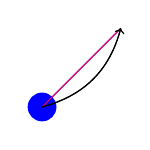
\begin{tikzpicture}
  \filldraw [blue] circle (5pt);
  \scopenode[draw=red, fill=orange, name=bob, at={(2,2)}, anchor=south west]{%
    \draw (0,0) coordinate (a) -- (1,1) coordinate (b);
  }
  \scopenode[draw=blue, fill=yellow, name=gog, at={(-2,-2)}, anchor=north east]{%
    \draw [magenta] (1,1) coordinate (c) -- (0,0) coordinate (d);
  }
  \draw [->] (a) [bend right] to (c);
  \draw [->] (d) [bend right] to (b);
\end{tikzpicture}
%
%
\ifdefined\DenKr\end{document}\else\DenKrTikzStandalonePost\fi%